\section{Your First Day}\label{sec:"Your First Day"}
It's your first day as Information Security Officer\resourcecite{WCISO}: everything is broken, servers are hacked, backups are failing, policies are missing, but somehow business goes on. Patients are still being treated. Financial transactions are still being processed. Take a deep breath. If security was easy, you would not have a job. You can make a difference. It will take time.\\\\The primary job of any information security personnel is to reduce risk; however, we often forget about this when we are lost in the details of a critical issue. This handbook is therefore written with a belief in risk management. You cannot eliminate all risks. If a high-risk issue that can be mitigated for cheap, do it. If you cannot justify the cost of a cool product, do not spend the money.\\\\
Before we get started, let me highlight one key for your program: transparency. Transparency in your program is important. Your leadership, coworkers, and customers all have an interest in your Information Security Program. Some security folks hide behind the auspices of security through obscurity\resourcecite{WSTO} and do not discuss their programs. This hurts their program and their organization. Sharing information about your program within your organization (and sometimes outside your organization) strengthens your program. It helps others know what resources are available to them, the benefits of your program, why they should care about your program, and why they should fund your program. These days large organizations such as Google\resourcecite{GVRPR} and Amazon\resourcecite{AWSSC} share information about their security programs publicly and even pay bounties to those who discover bugs in their software.\\\\
\textbf{Resources}
\begin{enumerate}
\resource[WCISO]{Chief information security officer - Wikipedia}{https://en.wikipedia.org/wiki/Chief_information_security_officer}
\resource[WSTO]{Security through obscurity - Wikipedia}{https://en.wikipedia.org/wiki/Security_through_obscurity}
\resource[GVRPR]{Google Vulnerability Reward Program (VRP) Rules}{https://www.google.com/about/appsecurity/reward-program/}
\resource[AWSSC]{Amazon Web Services (AWS) Security Center}{https://aws.amazon.com/security/}
\resource{Outline of computer security - Wikipedia}{https://en.wikipedia.org/wiki/Outline_of_computer_security}
\end{enumerate}
\subsection{Design, Leadership, and Education}
Design, Leadership, and Education are the three most important elements of your Information Security Program. However, these elements are often overlooked in otherwise strong Programs. This is likely because these three are core components of a Masters in Business Administration (MBA); they are not technical. Think of your Information Security Programs as an organization within the organization.\\\\
Design\resourcecite{WDoET} is the most important element of your Program because it is the most effective. Design your Program for everyone in your organization. Consider how every element of your Program interacts with every employee. This includes system administrators, developers, nontechnical coworkers, and you. Also consider those outside your organization. This is an opportunity to start from scratch.\\\\
Think outside the box when you design your Program. I had a great phone call with the Information Security Officer of a Federal organization a couple years ago. He was tired of the state of the industry: "I'm doing everything, I'm following all the best practices, and we still have problems." He was right. Even if you implement everything this handbook recommends, there is still a chance you will be hacked. Sometimes the best approach is to take a step back and redesign your Program from scratch.\\\\
Leadership is the second most important element of your Program. Leadership must believe in your Program and they must support your Program. Your job is to build a program they believe in and support. Support consists of financial resources, human resources, their own compliance with the Program, an email to all employees, etc. Your coworkers need to see support from leadership before they will believe in your Program.\\\\
Education is the third most important element of your Program. First, you need to educate yourself. Educate yourself on your organization: the culture, your coworkers, the policies, and the processes. One of the best ways to do this is with the Assessments. Please see \hyperref[sec:"Assessments, Audits, and Analyses"]{Assessments, Audits, and Analyses} for more information.\\\\
Educate yourself on Information Security. This handbook is a good educational resource, and it contains hundreds of references to other resources. Read books, blogs\resourcecite{KrebsonSecurity}, and websites\resourcecite{DM}\textsuperscript{,}\resourcecite{HackerNews}\textsuperscript{,}\resourcecite{Rnetsec}. Subscribe to mailing lists\resourcecite{USCERTMLF}\textsuperscript{,}\resourcecite{USNISTCSRC}. Watch videos\resourcecite{Lynda}. Listen to podcasts\resourcecite{SpiderLabsRadio}. Join chat rooms\resourcecite{IRCsecurity}. Test new tools. Attend conferences. Take classes\resourcecite{Coursera}\textsuperscript{,}\resourcecite{CourseraCSDomains}\textsuperscript{,}\resourcecite{SANS}. Follow people on Twitter. Join organizations.\resourcecite{ISACA}\textsuperscript{,}\resourcecite{OWASP} Write software. Learn from other organizations in your industry  by looking for at their websites and talking to their Information Security Officers. Educate yourself throughout your career.\\\\
Educate yourself on any laws and regulations that govern your organization. If you work in healthcare, read the HIPAA Security Rule\resourcecite{HIPAASR}. If you accept credit cards, read the Payment Card Industry Data Security Standards\resourcecite{PCIDSS}. These documents are dense and can be hard to read, but you must understand them yourself before you can effectively educate your coworkers. Build you Program with these laws and regulations in mind. 90\% of Information Security is the same in any industry. The 10\% that is different is in these laws and regulations.\\\\
Educate your coworkers.\resourcecite{STH}\textsuperscript{,}\resourcecite{SM} Every employee in your organization needs Information Security education. Design this education so it is appropriate for each employee and effective. Create different education programs for system administrators, developers, and other coworkers. Take everything you have learned about the organization, Information Security, and governing laws and regulations and teach it to your coworkers. Create a catalog of services offered by your Information Security Program.\resourcecite{StanfordIS}\\\\
Educate new employees during their on-boarding. Educate existing coworkers regularly. Educate terminated coworkers during their off-boarding. Please see \hyperref[subsec:"Employee Life Cycle"]{Employee Life Cycle} for more information.\\\\
There are many mediums for education for your employees. Create presentations and speak at meetings and events. Build a website for your Program. Create a library of books. Email newsletters and tips\resourcecite{SANSTips}. Provide tools and services to your organization. Send employees to training and conferences. Create or subscribe to online classes. Recommend mailing lists and websites. Create checklists and "one-pagers." Remember Marketing's Rule of Seven\resourcecite{RuleOf7}: your employees need to hear or see your message seven times before they will buy it. Use many mediums to communicate with your employees.\\\\
Design your education program with Plain Language\resourcecite{PlainLanguage}\textsuperscript{,}\resourcecite{PLAIN}\textsuperscript{,}\resourcecite{PlainEnglishHandbook}. Consider your audience and write for their needs. Clarify complex Information Security concepts, laws and regulations and make them understandable for your audience. Use active voice and positive language. Use simple words and short sentences. Use pictures, bullets, and other design elements to simplify your educational materials. Communicate with your users as they would communicate with themselves. Focus your education on one or two topics at a time. Test your educational materials with a subset of your intended audience. Plain language is one of the most important concepts in a successful program. This paragraph greatly summarizes the importance and implementation of plain language. Remember it is your job to translate complex concepts into understandable education.\\
\begin{mdframed}
\emph{Calvin: I used to hate writing assignments, but now I enjoy them. I realized that the purpose of writing is to inflate weak ideas, obscure poor reasoning, and inhibit clarity. With a little practice, writing can be an intimidating and impenetrable fog!}\\ -- Bill Watterson, Calvin and Hobbes: Homicidal Psycho Jungle Cat
\end{mdframed}\vspace{5mm}
Use Nudge theory\resourcecite{WNudge} to influence your organization's culture. For example, placing the shred bin in front of the trash can makes a difference in where your employees dispose of private information. Make your program visible, open, and honest.\\\\
The Anatomy of an Attack (included as an Appendix) is an example educational presentation. It is brief and suitable for most employees. It covers many high-risk topics and provides guidance for your employees. Customize it for your organization, add a bunch of examples (screenshots), and try it on your employees. Almost every information security company has a piece of marketing with the same title, the Anatomy of an Attack. This presentation is marketing for your Program.\\\\
Everyone is responsible for information security. With Design, Leadership, and Education, you can build information security into your organization's culture and everything your company does. Remember Design is the most effective element in your Program.\\\\
\textbf{Resources}
\begin{enumerate}
\resource[WDoET]{The Design of Everyday Things - Wikipedia}{https://en.wikipedia.org/wiki/The_Design_of_Everyday_Things}
\resource[KrebsonSecurity]{Krebs on Security}{https://krebsonsecurity.com}
\resource[DM]{Daniel Miessler}{https://danielmiessler.com}
\resource[HackerNews]{Hacker News}{https://news.ycombinator.org}
\resource[Rnetsec]{Reddit /r/netsec - Information Security News \& Discussion}{https://reddit.com/r/netsec}
\resource[USCERTMLF]{US-CERT Mailing Lists and Feeds}{https://www.us-cert.gov/mailing-lists-and-feeds}
\resource[USNISTCSRC]{NIST Computer Security Resource Center Mailing List}{https://public.govdelivery.com/accounts/USNISTCSRC/subscriber/new}
\resource[Lynda]{Lynda.com: Online Video Tutorials \& Training}{https://www.lynda.com}
\resource[SpiderLabsRadio]{SpiderLabs Radio}{https://www.trustwave.com/Resources/SpiderLabs-Radio/}
\resource[IRCsecurity]{\#\#security on freenode}{irc://irc.freenode.net/\#\#\#\#security}
\resource[Coursera]{Coursera - Computer Science: Systems \& Security}{https://www.coursera.org/courses?categories=cs-systems}
\resource[CourseraCSDomains]{Coursera - Cybersecurity and Its Ten Domains}{https://www.coursera.org/learn/cyber-security-domain}
\resource[SANS]{SANS}{https://www.sans.org}
\resource[ISACA]{ISACA}{https://www.isaca.org}
\resource[OWASP]{Open Web Application Security Project}{https://www.owasp.org}
\resource[HIPAASR]{HIPAA Security Rule}{http://www.hhs.gov/ocr/privacy/hipaa/administrative/securityrule/securityrulepdf.pdf}
\resource[PCIDSS]{Payment Card Industry (PCI) Data Security Standards (DSS)}{https://www.pcisecuritystandards.org/documents/PA-DSS_v3.pdf}
\resource[STH]{STH.EndUser Security Awareness Training}{https://securingthehuman.sans.org/enduser/}
\resource[SM]{Security Mentor}{https://www.securitymentor.com}
\resource[StanfordIS]{Stanford Information Security}{https://itservices.stanford.edu/security}
\resource[SANSTips]{Security Awareness Tip of The Day}{https://www.sans.org/tip_of_the_day.php}
\resource[RuleOf7]{Your Brand and the Marketing Rule of 7}{http://thewordchef.com/2011/12/your-brand-and-the-marketing-rule-of-7/}
\resource[PlainLanguage]{Plain Language: Improving Communications from the Federal Government to the Public}{http://www.plainlanguage.gov}
\resource[PLAIN]{Plain Language Association International}{http://www.plainlanguagenetwork.org}
\resource[PlainEnglishHandbook]{A Plain English Handbook: How to create clear SEC disclosure documents}{http://www.sec.gov/pdf/handbook.pdf}
\resource[WNudge]{Nudge theory - Wikipedia}{https://en.wikipedia.org/wiki/Nudge_theory}
\end{enumerate}
\subsection{Risk Management}
\begin{mdframed}
\emph{Risk Management: It's Not Rocket Science...It's Much More Complicated}\\ -- John Adams
\end{mdframed}
Risk Management\resourcecite{80039}\textsuperscript{,}\resourcecite{WITRM}\textsuperscript{,}\resourcecite{FISSISRM}\textsuperscript{,}\resourcecite{FAIRWIKI} is Economics, the study of scarcity, applied to Information Security. What is Risk? Like other terms in Information Security, Risk has many definitions. Most people think of risk as...
\begin{equation}
Risk = Something\ Bad\ That\ Can\ Happen
\end{equation}
This is a good definition for informal conversations. However, we need to formalize risk. When we change "Something Bad" to Impact and "Can Happen" to Probability, risk is...
\begin{equation}
Risk = Probability * Impact
\end{equation}
This is a powerful, mathematical definition that we can apply almost anywhere. With this definition, impact can be positive or negative. We can use this definition for decision making by making Pros and Cons lists. Below is an example of the Pros and Cons of increasing required password length from 8 characters to 12 characters.\\\\
\begin{tabularx}{\textwidth}{ X | X }
Pros & Cons\\\hline
Reduced probability of a successful brute-force password attack & Increased probability of users forgetting their passwords\\
 & Increased probability of users writing down their passwords
\end{tabularx}\vspace{5mm}
Here we see that increasing the required password length may not make the system more secure depending on these probabilities. Risk Management balances both sides of a decision. Formal Risk Management programs outside Information Security, such as those that manage financial risk\resourcecite{WFinRisk}, are based on this approach. Consider financial risk and other risks such as employee happiness when making decisions. However, when we add the idea of an threat source exploiting a vulnerability, risk is...
\begin{align}
Risk &= The\ Probability\ a\ Threat\ Source\ Exploits\ a\ Vulnerability \nonumber \\ &\ * The\ Impact\ of\ the\ Vulnerability\ Being\ Exploited
\end{align}
This is the formal definition of Risk for Information Security Programs. NIST SP 800-30 Guide for Conducting Risk Assessments\resourcecite{80030} defines Risk as above with the Risk Model (Figure~\ref{fig:RiskModel}).
\begin{figure}[ht]
\centering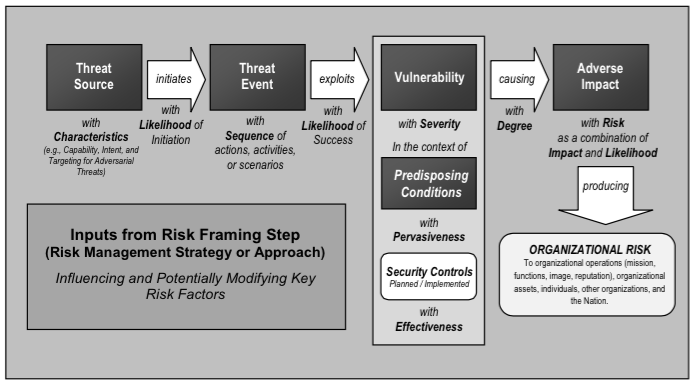
\includegraphics[scale=.55]{./img/RiskModel}
\caption{Risk Model (NIST Special Publication 800-30 Revision 1)}
\end{figure}\label{fig:RiskModel}
The impact of all Information Security risks falls into at least one of three categories:
\begin{itemize}
\item Confidentiality - information can be inappropriately accessed
\item Integrity - information can be inappropriately changed  
\item Availability - information can be made unavailable
\end{itemize}
Confidentiality, Integrity, and Availability are called the CIA triad. Using our example above, you can increase the confidentiality of a system by increasing the required password length, but this can decrease the availability of the system when users forget their passwords. Conversely, you can increase the availability of a system by decreasing the required password length, but this can decrease the confidentiality of the system when attackers successfully brute-force a password. We often forget Integrity in Risk Management, but what good is the information if you can’t trust it to be accurate?\\\\
Using the above definition of risk, NIST SP 800-37 Security and Privacy Controls for Federal Information Systems and Organizations\resourcecite{80037} creates a six step Risk Management Framework\resourcecite{RMFramework} (Figure~\ref{fig:RiskManagementFramework}) that defines a Security Life Cycle for your Information Security Program. Throughout this handbook, we will apply this framework to your organization.
\begin{figure}[ht]
\centering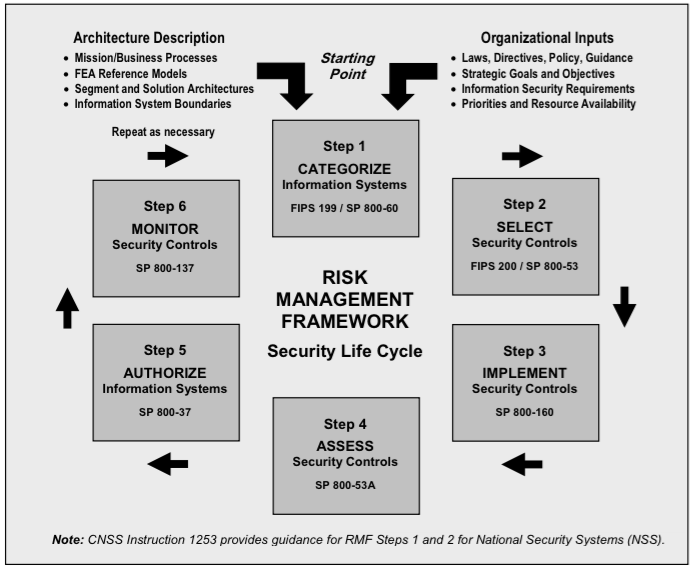
\includegraphics[scale=.55]{./img/RiskManagementFramework}
\caption{Risk Management Framework (NIST Special Publication 800-37 Revision 1)}\label{fig:RiskManagementFramework}
\end{figure}
The steps of the Risk Management Framework are:
\begin{enumerate}
\item Categorize the information system and the information processed, stored, and transmitted by that system based on an impact analysis.
\item Select an initial set of baseline security controls for the information system based on the security categorization; tailoring and supplementing the security control baseline as needed based on an organizational assessment of risk and local conditions.
\item Implement the security controls and describe how the controls are employed within the information system and its environment of operation.
\item Assess the security controls using appropriate assessment procedures to determine the extent to which the controls are implemented correctly, operating as intended, and producing the desired outcome with respect to meeting the security requirements for the system.
\item Authorize information system operation based on a determination of the risk to organizational operations and assets, individuals, other organizations, and the Nation resulting from the operation of the information system and the decision that this risk is acceptable.
\item Monitor the security controls in the information system on an ongoing basis including assessing control effectiveness, documenting changes to the system or its environment of operation, conducting security impact analyses of the associated changes, and reporting the security state of the system to designated organizational officials.
\end{enumerate}
The next section, Information Classification, introduces the concept of categorization. Every section of this handbook contains controls for you to select, implement, assess, and monitor. Chapter 3, Assessments, Audits, and Analyses, details how to assess the security controls you have selected and implemented. Leadership, the second most important element of your Program is responsible for Authorization in your organization.\\\\
Risk management is a powerful tool for your organization because it allows you to formalize and contextualize risk. Use Risk to choose between two projects competing for your time and budget. Use Risk to develop a budget for your Information Security Program. Use Risk to weigh action versus inaction.\\
\begin{mdframed}
"The Goldman Sachs risk system is called SecDB (securities database), and everything at Goldman that matters is run out of it."\resourcecite{SecDB}
\end{mdframed}\vspace{5mm}
\textbf{Resources}
\begin{enumerate}
\resource[80039]{NIST Special Publication 800-39: Managing Information Security Risk - Organization, Mission, and Information System View}{http://csrc.nist.gov/publications/nistpubs/800-39/SP800-39-final.pdf}
\resource[WITRM]{IT Risk Management - Wikipedia}{https://en.wikipedia.org/wiki/IT_risk_management}
\resource[FISSISRM]{Fundamentals of Information Systems Security/Information Security and Risk Management}{https://en.m.wikibooks.org/wiki/Fundamentals_of_Information_Systems_Security/Information_Security_and_Risk_Management}
\resource[FAIRWIKI]{FAIRWIKI: The Definitive Guide to the Factor Analysis of Information Risk (FAIR)}{http://fairwiki.riskmanagementinsight.com}
\resource[WFinRisk]{Financial risk - Wikipedia}{https://en.wikipedia.org/wiki/Financial_risk}
\resource[80030]{NIST Special Publication 800-30 Revision 1: Guide for Conducting Risk Assessments}{http://csrc.nist.gov/publications/nistpubs/800-30-rev1/sp800_30_r1.pdf}
\resource[80037]{NIST Special Publication 800-37 Revision 1: Guide for Applying the Risk Management Framework to Federal Information Systems - A Security Life Cycle Approach}{http://csrc.nist.gov/publications/nistpubs/800-37-rev1/sp800-37-rev1-final.pdf}
\resource[RMFramework]{Risk Management Framework Overview - NIST CSRC}{http://csrc.nist.gov/groups/SMA/fisma/framework.html}
\resource[SecDB]{Why founding a three-person startup with zero revenue is better than working for Goldman Sachs.}{http://blogs.itb.ac.id/djadja/2010/09/15/why-founding-a-three-person-startup-with-zero-revenue-is-better-than-working-for-goldman-sachs-adgrok/}
\end{enumerate}
\subsection{Information Classification}
Information Classification allows us to create different classes of information with different protections. First we will create two different classes of information and then we will determine how to protect those classes.
\begin{description}
\item\textbf{Public Information}\\ Public information is information you would share with everyone. Availability is more important than Confidentiality. In fact, Confidentiality has no importance. Integrity is important. Example availability and integrity risks include a web server that is unavailable or defaced.
\item\textbf{Private Information}\\ Private information is all information that is not public. Other names for this classification include need-to-know, confidential, and proprietary. Confidentiality is more important that Availability. Integrity is important.
\end{description}
This may seem obvious: there is information that we must protect (private) and information that we do not need to protect (public). However, this is the basis of Information Security. Each classification has subclasses specific to your organization. Be clear about what information belongs in each class or subclass. The rest of this handbook describes how we protect these classes of information.\\\\Most laws and regulations use specific data elements to define their classes. HIPAA defines Protected Health Information\resourcecite{WPHI}, PCI defines Account Data, and California SB1386\resourcecite{WSB1386} defines Personally identifiable information\resourcecite{WPII}. Many universities\resourcecite{Harvard}\textsuperscript{,}\resourcecite{CMU}\textsuperscript{,}\resourcecite{Stanford} publish comprehensive data classification matrices. We will talk more about specific laws and regulations in \hyperref[sec:"Policies and Processes"]{Policies and Processes}.\\\\
\textbf{List of Protected Health Information (PHI) Identifiers}\resourcecite{PHI}
\begin{enumerate}
\item Names
\item All geographical identifiers smaller than a state, except for the initial three digits of a zip code if, according to the current publicly available data from the Bureau of the Census: the geographic unit formed by combining all zip codes with the same three initial digits contains more than 20,000 people; and [t]he initial three digits of a zip code for all such geographic units containing 20,000 or fewer people is changed to 000
\item All elements of dates (except year) for dates directly related to an individual, including birth date, admission date, discharge date, date of death; and all ages over 89 and all elements of dates (including year) indicative of such age, except that such ages and elements may be aggregated into a single category of age 90 or older;
\item Phone numbers
\item Fax numbers
\item Email addresses
\item Social Security numbers
\item Medical record numbers
\item Health insurance beneficiary numbers
\item Account numbers
\item Certificate/license numbers
\item Vehicle identifiers and serial numbers, including license plate numbers;
\item Device identifiers and serial numbers;
\item Web Uniform Resource Locators (URLs)
\item Internet Protocol (IP) address numbers
\item Biometric identifiers, including finger, retinal and voice prints
\item Full face photographic images and any comparable images
\item Any other unique identifying number, characteristic, or code except the unique code assigned by the investigator to code the data
\end{enumerate}
\textbf{Table of PCI Identifiers}\resourcecite{PCIDSSI}\\\\
\begin{tabularx}{\textwidth}{| X | X |}
\hline
\multicolumn{2}{| c |}{\textbf{Account Data}} \\
\hline
\textbf{Cardholder Data} & \textbf{Sensitive Authentication Data}\\
\hline
Primary Account Number (PAN) & Full track data (magnetic-stripe\\
Cardholder Name & data or equivalent on a chip)\\
Expiration Date & CAV2/CVC2/CVV2/CID\\
Service Code & PINs/PIN blocks\\
\hline
\end{tabularx}
\\\\\\ 
\textbf{California SB1386}\resourcecite{CASB1386}
\begin{description}
\item(e) For purposes of this section, "personal information" means an individual's first name or first initial and last name in combination with any one or more of the following data elements, when either the name or the data elements are not encrypted: (1) Social security number. (2) Driver's license number or California Identification Card number. (3) Account number, credit or debit card number, in combination with any required security code, access code, or password that would permit access to an individual's financial account. (f) For purposes of this section, "personal information" does not include publicly available information that is lawfully made available to the general public from federal, state, or local government records.
\end{description}
\textbf{Resources}
\begin{enumerate}
\resource[WPHI]{Protected health information - Wikipedia}{https://en.wikipedia.org/wiki/Protected_health_information}
\resource[WSB1386]{California S.B. 1386 - Wikipedia}{https://en.wikipedia.org/wiki/SB_1386}
\resource[WPII]{Personally identifiable information - Wikipedia}{https://en.wikipedia.org/wiki/Personally_identifiable_information}
\resource[Harvard]{Data Classification and Examples (abridged version) - Harvard University}{http://security.harvard.edu/files/it-security-new/files/data_classification_table_abridged_7.23.13_0.pdf}
\resource[CMU]{Guidelines for Data Classification - Carnegie Mellon University}{http://www.cmu.edu/iso/governance/guidelines/data-classification.html}
\resource[Stanford]{Data Classification, Access, Transmittal, and Storage - Stanford University}{http://web.stanford.edu/group/security/securecomputing/dataclass_chart.html}
\resource[PHI]{45 CFR 164.514 - Other requirements relating to uses and disclosures of protected health information.}{http://www.law.cornell.edu/cfr/text/45/164.514}
\resource[PCIDSSI]{Payment Card Industry (PCI) Data Security Standard}{https://www.pcisecuritystandards.org/documents/PCI_DSS_v3.pdf}
\resource[CASB1386]{SB 1386}{http://www.leginfo.ca.gov/pub/01-02/bill/sen/sb_1351-1400/sb_1386_bill_20020926_chaptered.html}
\end{enumerate}
\subsection{Information Inventory and Data Flow Diagrams}
Now that we have defined what information is public and private, we need to inventory it. Ideally we would have an application that automatically tracks every bit of information on every computer within the organization. Some Data Loss Prevention (DLP) software even claims to do this. (Please see \hyperref[subsubsec:"Data Loss Prevention"]{Data Loss Prevention} for more on DLP.) However, there are some more basic approaches. Many organizations use spreadsheets to keep inventories of where information is stored throughout the organization. These can be inflexible and hard to maintain for all but the smallest organizations. I personally prefer data flow diagrams to track information.\\\\
Data flow diagrams\resourcecite{WDFD} are a pictorial representation of where information is created in your organization and where that information travels. They include both storage and transmission of information. Because they can be limited to one type or source of information, they are great for visualizing the entire life of a bit of information. A collection of diagrams can represent all the information in your organization. They are also flexible enough to include arbitrary stores like email, file servers, and printed paper. Last, and most important, data flow diagrams help us  assess risk to data and implement the proper controls to mitigate that risk. Data flow diagrams can be created on whiteboards, paper, or software like Microsoft Visio, Dia, or DOT\resourcecite{WDOT}. A few basic data flows are below.\\\\
\begin{figure}[h]
\centering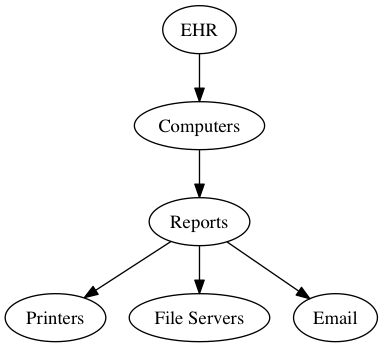
\includegraphics[scale=.75]{./img/ehrDataFlow}
\caption{A basic data flowing showing PHI that originates from the Electronic Health Record (EHR).}
\end{figure}
\begin{figure}[h]
\centering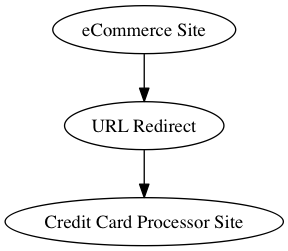
\includegraphics[scale=.75]{./img/eCommerceDataFlow}
\caption{A basic data flow showing credit card information.}
\end{figure}
\newpage
\textbf{Resources}
\begin{enumerate}
\resource[WDFD]{Data flow diagram - Wikipedia}{https://en.wikipedia.org/wiki/Data_flow_diagram}
\resource[WDOT]{DOT (graphic description language) - Wikipedia}{https://en.wikipedia.org/wiki/DOT_(graph_description_language}
\end{enumerate}
\subsection{About this Handbook}
Hopefully you have survived your first day as an Information Security Officer. Read on as we dig into the different areas of Information Security.\\\\
My goal for this handbook is to create an introduction to Information Security and a reference. Please be free to edit sections to better match your organization. Staple in your own organization's documentation for quick reference. Bring this handbook to meetings as a quick reference. Use the appendices to perform your own assessments. Write me (david@davidabailey.com) with your suggestions. Hopefully this book is valuable to everyone from those who are just getting started to Chief Information Security Officers.\\\\
This handbook focuses on the healthcare industry and often uses examples from NIST, HIPAA, and PCI. However, most other regulated industries have similar requirements. The principles of this handbook should apply to all information security programs.\\\\I designed this handbook with vendor neutrality in mind. Vendor selection is often a hostile topic. It is up to your organization to select the vendors and products. The only advise I can give is to disclose and avoid conflicts of interest. There is a lot of BS in the information security world, and it can be hard to make sense of everything. Just remember spending money is not always the best solution, and spending more money is not always better. We tell ourselves we can mitigate all our risk if only we had more money. We get that warm and fuzzy feeling after spending a lot of money. These are false. Money helps, but it is not everything.\\\\
One last thing to remember before we get going is that any or all of you Information Security Program, just like the rest of your business, can be outsourced. It is up to you and your organization to determine when to outsource. Most organizations keep a balance of inside versus outside.\\\\This hand book is structured from high-level to low-level, abstract to concrete, both in terms of information security and organizational structure. Sections build on previous section, but are also designed to be independent. Don't hesitate to jump ahead.\\\\
\textbf{Sections}
\begin{description}
\item \hyperref[sec:"Policies and Processes"]{Policies and Processes}
\item \hyperref[sec:"Assessments, Audits, and Analyses"]{Assessments, Audits, and Analyses}
\item \hyperref[sec:"Networks"]{Networks}
\item \hyperref[sec:"Computers"]{Computers}
\item \hyperref[sec:"Identity and Access Management"]{Identity and Access Management}
\item \hyperref[sec:"Cryptography"]{Cryptography}
\item \hyperref[sec:"Physical"]{Physical}
\end{description}\vspace{5mm}
Each section and subsection of this handbook ends with additional information about the topic where appropriate:
\begin{description}
\item\textbf{Assessment} lists steps for you to evaluate your Information Security Program's effectiveness in this section. This section can be used to build security assessments described in \hyperref[sec:"Assessments, Audits, and Analyses"]{Assessments, Audits, and Analyses}.
\item\textbf{Documentation} lists the relevant documentation your organization needs to address this section. 
\item\textbf{Risk Management} lists the Threats and Controls applicable to this section. This section is a starting point for your risk assessment. 
\item\textbf{Resources} provide additional information about the topics covered in this section. Occasionally there are links to how other organizations are addressing the topic.
\item\textbf{Stories} is a collection of real-life events that highlight risks present in this section. These stories help reiterate the importance of the section to your organization. They are also useful for conveying the importance of your Information Security Program to leadership. Last they provide scenarios for your education program. 
\end{description}